\section{Modulo Zonas Turísticas}

\subsection{Objetivo}
El objetivo de este módulo es poder registrar, las zonas geográficas asocindoles un nombre, puntuación, descripción, estado, imagenes y delimitación geográfica.

\subsection{Diseño}

Para éste módulo se desarrolló en Node JS una interfaz gráfica web para que el administrador pueda gestionar las zonas turísticas y su información relacionada

\subsection{Desarrollo}

Para el desarrollo de la vista se tomo como base una plantilla HTML con CSS y para el controlador se utilizo Node JS para implementar un endpoint donde se almacena la información de las zonas turísticas.

\subsection{Resultados}

La Figura \ref{fig:zonas} muestra la pantalla principal donde se enlistan y gestionan las zonas turísticas, así mismo en la figura \ref{fig:agregar} se observa la pantalla correspondiente al ingreso de la información de una zona turística.\\

\begin{figure}[htbp]
	\begin{center}
		\fbox{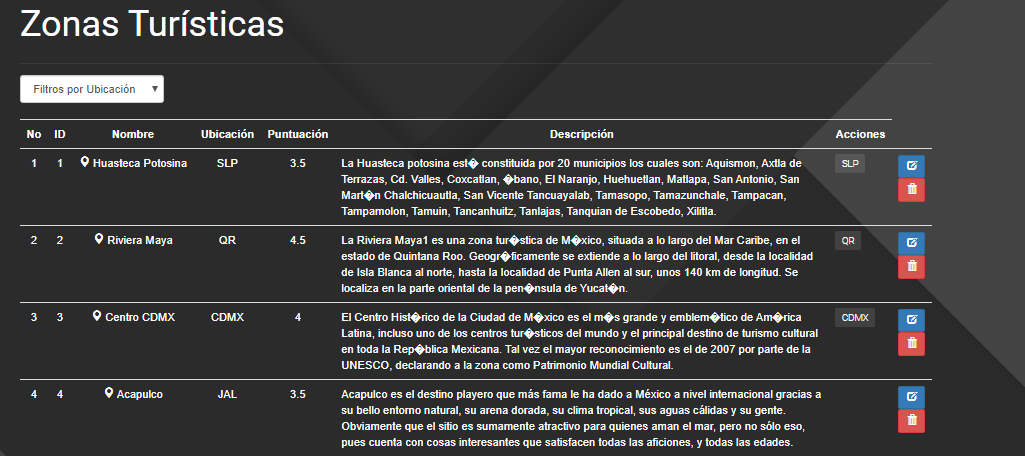
\includegraphics[scale = .6]{implementacion/zonas/images/zonas}}
		\caption{Gestión de Zonas Turísticas}
		\label{fig:zonas}
	\end{center}
\end{figure}

\begin{figure}[htbp]
	\begin{center}
		\fbox{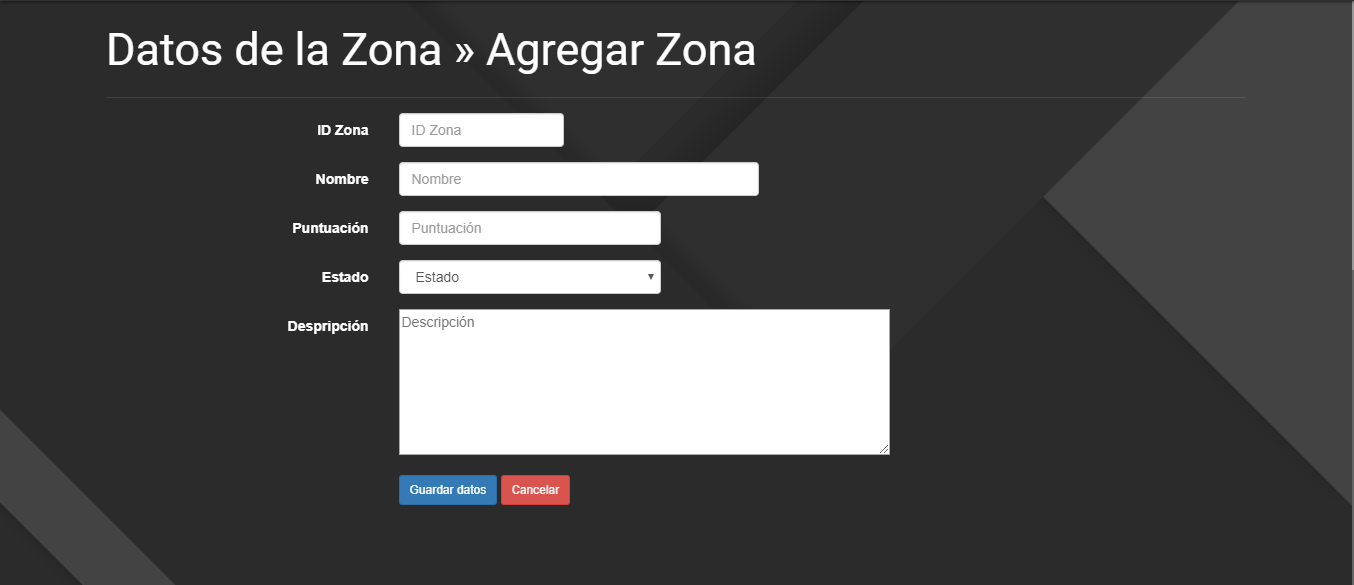
\includegraphics[scale = .5]{implementacion/zonas/images/agregar}}
		\fbox{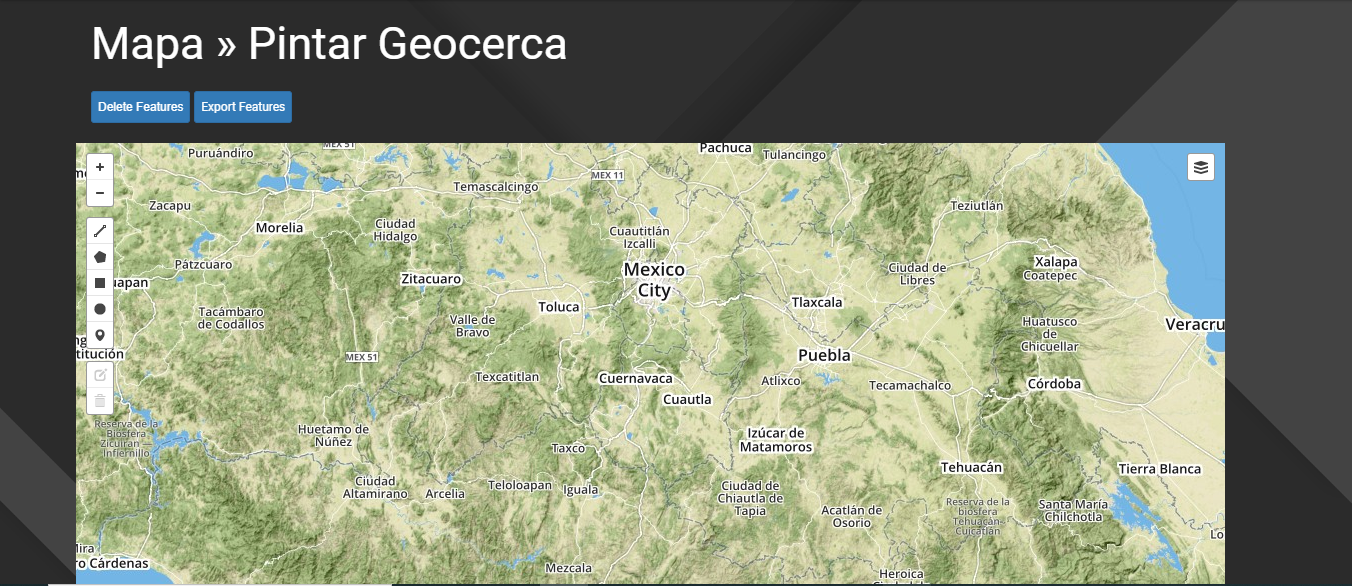
\includegraphics[scale = .5]{implementacion/zonas/images/mapa}}
		\caption{Agregar Zona Turística}
		\label{fig:agregar}
	\end{center}
\end{figure}



